\chapter{Conclusions et perspectives}
\label{chap:conclusion}

\section{Discussion générale}

Dans le cadre de cette thèse, nous sommes partis du constat que, si la littérature traite de l'accessibilité des milieux urbains aux \gls{pcdv}, peu d'études se sont spécifiquement intéressées aux carrefours. Or, ces espaces sont particulièrement critiques pour les personnes déficientes visuelles et nécessitent des compétences avancées en orientation et mobilité pour les traverser en sécurité \cite{ratelle_manuel_2019}. Par ailleurs, s'il existe des dispositifs mobiles permettant de s'orienter au cours d'un trajet, les seules manières d'étudier un lieu ex-situ (et à fortiori un carrefour) restent la description ad-hoc par une personne tierce ou l'utilisation de cartes en relief. Il s'agit également d'un problème pour les \gls{ia} lors de séance de locomotion: l'étude d'un nouveau terrain implique la préparation manuelle de cartes en relief et de descriptions adaptées aux besoins de la personne accompagnée, ce qui peut être chronophrage. Pour répondre à ces problématiques, nous avons souhaité aborder le problème sous l'angle de la modélisation du carrefour du point de vue d'un piéton déficient visuel pour, à minima, en proposer une description textuelle, mais potentiellement répondre également à d'autres usages.

\newpar{}

% Modélisation

Dans un premier temps, nous nous sommes intéressés à la définition du carrefour du point de vue du piéton, et nous avons estimé qu'il s'agissait d'un espace délimité par des passages piétons. Sur cette base, nous avons proposé une définition du carrefour sous la forme d'un graphe géographique qui modélise notamment les branches du carrefours et les traversées piétonnes de celles-ci. Nous nous sommes par la suite intéressé à la possibilité de générer un tel graphe depuis \gls{osm}, en analysant ses possibilités et les données actuellement renseignées, et en proposant un modèle de données objet pouvant accueillir ces informations et faciliter leur manipulation. Nous avons étudié l'instanciation de ce modèle depuis \gls{osm} au travers d'une méthode de segmentation des carrefours au sein d'un graphe routier, élaborée à partir de la définition établie précédemment. Enfin, nous avons proposé des méthodes de complétion de ce graphe de carrefour pour permettre son analyse du point de vue de sa traversée par un piéton.

\newpar{}

% Description

Dans un second temps, nous nous sommes intéressés aux possibilités offertes par le modèle de carrefour conçu précédemment pour décrire textuellement un carrefour. Cependant, les besoins des personnes concernés et des instructeurs étant très variés, il est nécessaire de concevoir une chaîne permettant cette variabilité dans le fond et la forme du texte. Pour répondre à cette problématique, nous avons proposé un cadre générique de génération de description textuelle d'objets géographiques au sein d'un \gls{sig}. Ce cadre, inspiré de la littérature <<~donnée vers texte~>> repose sur la conception de patrons textuels pour définir la forme que prendra le texte pour chaque donnée. Dans une étape d'assemblage du document final, nous définissons un plan de description ou chaque patron est sélectionné et ordonné selon la sortie souhaité. Nous avons proposé l'application de ce cadre à la description de carrefour et avons souligné l'intérêt d'insérer un géomaticien dans la chaîne de conception de description pour implémenter techniquement les textes établis par les instructeurs. Nous avons également proposé d'autres cas d'utilisation appliqués à l'intégration de ces descriptions dans des mediums interactifs.

\newpar{}

% Expérimentation

Par la suite, nous avons présenté les implémentations des méthodes évoquées précédemment et fourni des exemples de résultats. Nous avons implémenté les méthodes de segmentation du carrefour et de complétion de données piétonnes en Python sous la forme des modules crseg et crmodel. Ces derniers ont été embarqués en entrée de la chaîne technique de génération de description textuelle réalisée sous le \gls{sig} QGIS. Pour cette dernière, nous avons implémenté deux boîtes à outils permettant d'une part de définir un patron par couche, et d'autre part d'assembler ces patrons au sein d'un document avec un système de sélection du patron adapté. Nous avons mobilisé cette chaîne pour la génération de quatre types de descriptions de carrefour adaptées à différents mediums, usages, et niveau d'interactivité. 

\newpar{}

Enfin, nous avons proposé d'évaluer les différents dispositifs conçus lors de nos travaux. Nous avons tout d'abord évalué les outils de segmentation de carrefour crseg et de complétion de données piétonnes crmodel en comparant leurs résultats à un œil expert sur plusieurs échantillons de carrefours. Pour le premier, cela nous a permis de valider le fonctionnement de la méthode et d'estimer sa sensibilité aux paramètres et à la donnée en entrée. Nous avons pu voir pour le second que la qualité du résultat était particulièrement dépendante de la complétude des données \gls{osm} en entrée. Par la suite, nous nous sommes intéressés à la capacité de la chaîne de description à s'adapter à des besoins variés. Pour cela, nous avons émis un questionnaire à des \gls{ia} pour collecter des modifications du plan de description originellement établi. Nous avons catégorisé ces modifications, et pour chacune nous avons évalué la possibilité de les intégrer dans la chaîne de génération de description.

\section{Perspectives}

Dans cette dernière partie, nous allons discuter des perspectives ouvertes par nos travaux et des pistes de recherche futures.

\subsection{Vers des données plus précises}

Depuis le début de nos travaux, les questions autour de la mobilité des personnes concernées par un handicap ont pris une place importante dans le débat public. En particulier, la \gls{lom} promulguée en 2019 a introduit de nouvelles obligations pour les gestionnaires de voirie, dont la collecte et la mise à disposition de données d'accessibilité de la voirie et des réseaux à deux cents mètres autour des arrêts de transport en commun. Ces données, fournies dans un format standardisé par le \gls{cnig} \citep{geostandard2021} qui étend le format \gls{netex}, visent une précision très grande dans la description des cheminements piétons (voir figure \ref{fig:conclusion_exemple_lom}). Si la disponibilité de ces données est encore parcellaire, elles pourraient à terme devenir une source de données privilégiée pour étendre et préciser les capacités de description de carrefour que nous avons proposées. Des travaux préliminaires menés par \citet{WadjomKammegne2021} s'intéressent à la compatibilité entre le modèle du \gls{cnig} et celui d'\gls{osm}, et pourraient servir de base à une intégration de ces données dans notre modèle.

\begin{figure}[ht]
    \centering
    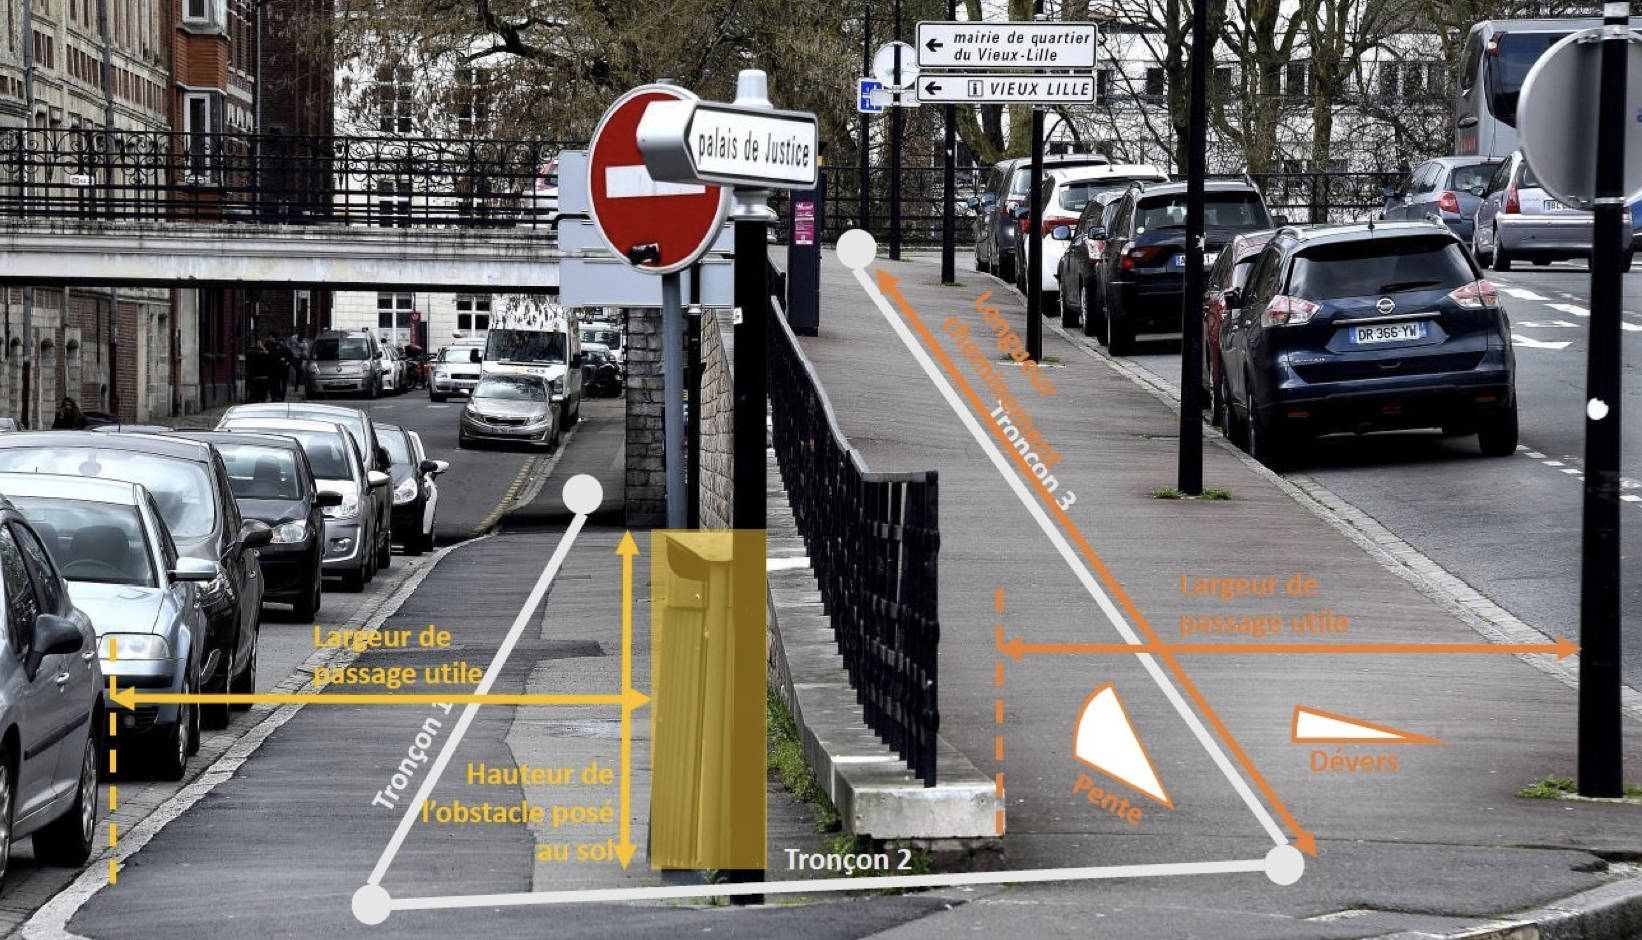
\includegraphics[width=\textwidth]{images/conclusion/graphe_geostandard.png}
    \caption[Graphe de cheminement du géostandard]{Exemple de graphe pouvant correspondre à un cheminement décrit dans le formalisme du géostandard accessibilité du \gls{cnig}. Source: \citep{geostandard2021}.}
    \label{fig:conclusion_exemple_lom}
\end{figure}

\newpar{}

Par ailleurs, un intérêt particulier autour de l'accessibilité ces dernières années amènent les données \gls{osm} à s'améliorer constamment. Outre les évolutions autour de la sémantique permettant une description plus fine des infrastructures\footnote{https://wiki.openstreetmap.org/wiki/Proposal:Crossing:markings}\footnote{https://wiki.openstreetmap.org/wiki/Proposal:Key:is\_sidepath}, l'émergence de nouveaux outils spécialisés pour améliorer les données autour de l'accessibilité comme EveryDoor\footnote{https://wiki.openstreetmap.org/wiki/Every\_Door} ou OSM Sidewalkreator \citep{demoraesvestena2023} contribuent à une accélération de la cartographie de ces informations.

\subsection{Aller au-delà du carrefour}

Dans les travaux présentés dans ce manuscrit, nous avons essentiellement travaillé sur les carrefours en tant qu'objets isolés. Il s'agit cependant d'étapes qui s'inscrivent au sein d'un itinéraire \citep{gaunet_verbal_2006} plus large dans la ville, or les descriptions que nous produisons ne recontextualisent pas les carrefours en dehors des noms de rues (voir chapitre \ref{chap:description}). Une proposition que nous avions émise dans le <<~carrefour dont vous êtes le héros~>> (voir \ref{sec:experimentation_le_carrefour_dont_vous_etes_le_heros}) était d'associer une direction à une branche, sous la forme d'un point d'intérêt connu au sein de la ville. Déterminés manuellement dans cette expérimentation, ces points d'intérêt pourraient être extraits automatiquement. Des travaux préliminaires ont été menés par \citet{aouini2023} qui propose de sélectionner pour chaque branche le point d'intérêt (parmi une préselection de type d'entité) le plus proche selon la distance de Manhattan et la direction pointé par la branche (voir figure \ref{fig:conclusion_exemple_ali}).

\begin{figure}[ht]
    \centering
    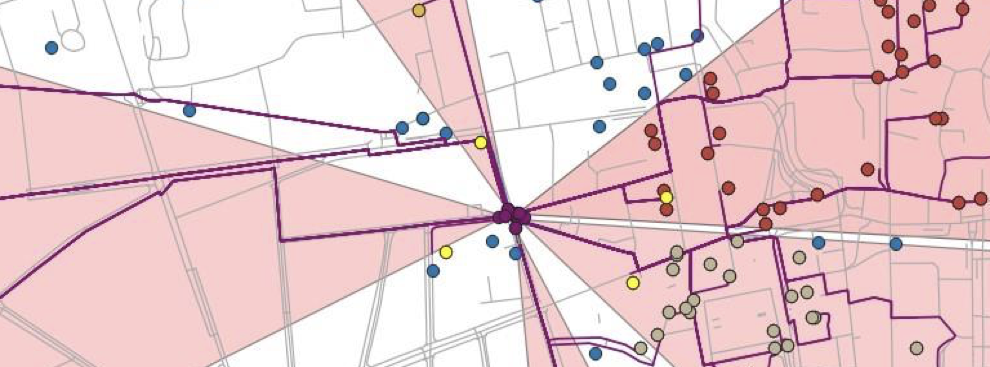
\includegraphics[width=\textwidth]{images/conclusion/stage_ali.png}
    \caption[Labellisation des branches d'un carrefour]{Exemple de résultat obtenu par la méthode proposée par \citet{aouini2023} pour labelliser les branches d'un carrefour. Source: \citep{aouini2023}.}
    \label{fig:conclusion_exemple_ali}
\end{figure}

\newpar{}

Par ailleurs, si nous nous sommes concentrés sur la description des carrefours, ces derniers peuvent être un point de départ à la description de quartiers. C'est le travail amorcé par \citet{guillaumin2023} qui s'intéressent à la description du chemin entre les carrefours. Ils proposent d'utiliser les résultats fournis par crseg et de considérer les carrefours comme des nœuds. Les arêtes du graphe de quartier sont alors les branches des carrefours étendues jusqu'au prochain carrefour (voir figure \ref{fig:conclusion_exemple_chemin_carrefour}). Cette approche permet de décrire des quartiers entiers, et de proposer des itinéraires en utilisant les carrefours comme points de passage.

\begin{figure}[ht]
    \centering
    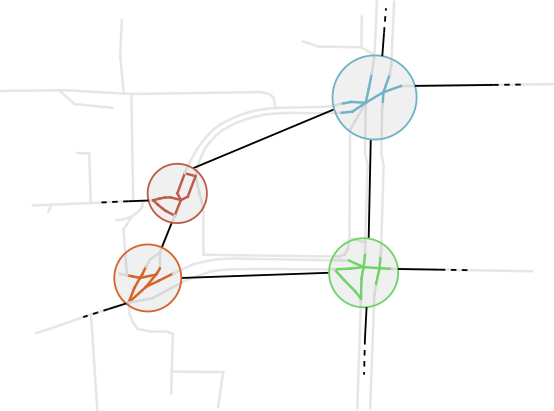
\includegraphics[width=0.7\textwidth]{images/conclusion/chemin_carrefour.png}
    \caption[Graphe de quartier]{Exemple d'un graphe de quartier. Les carrefours deviennent des nœuds liés entre eux par leurs branches.}
    \label{fig:conclusion_exemple_chemin_carrefour}
\end{figure}


\subsection{Les apports de l'intelligence artificielle}

Au début de nos travaux, nous avons fait le choix pour la génération de texte de nous reposer sur la méthode des patrons textuels, classiques dans le domaine <<~données vers texte~>> (voir chapitre \ref{chap:description}). Notre objectif à travers ce choix était notamment de s'assurer de la fiabilité de la mise en forme du texte définie par le plan de description, les intelligences artificielles génératives étant promptes aux <<~hallucinations~>> \citep{ye2023} et aux erreurs d'interprétation (voir figure \ref{fig:conclusion_dallemini}). Par ailleurs, il n'existait aucun corpus de description de carrefour pour entraîner un modèle.

\begin{figure}[ht]
    \centering
    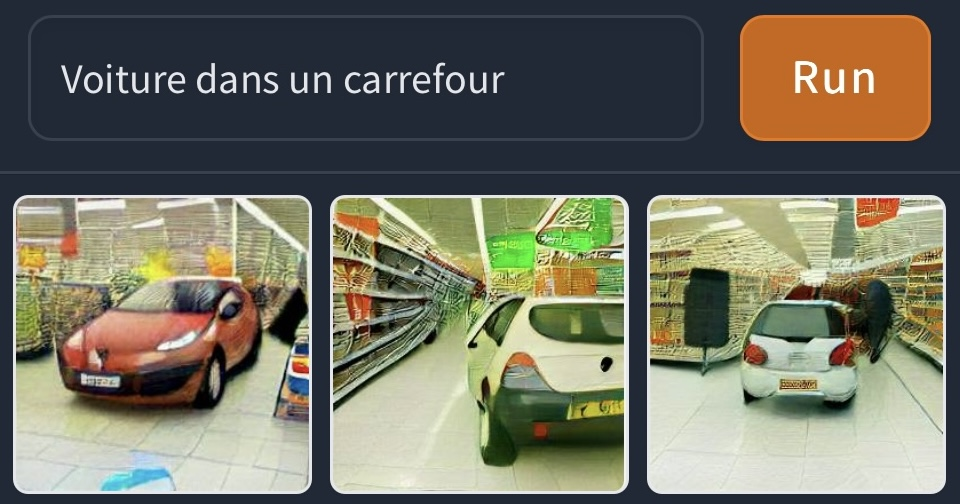
\includegraphics[width=0.5\textwidth]{images/conclusion/dallemini_voiture.jpeg}
    \caption[Une voiture dans un carrefour]{Exemple d'image obtenue avec DALL-E Mini en juin 2022.}
    \label{fig:conclusion_dallemini}
\end{figure}

Cependant, cela rend la création d'un patron particulièrement lourde pour l'utilisateur, et nécessite une expertise techniques pour sa mise en œuvre. Notamment, notre approche nécessite l'usage d'un réalisateur de texte pour segmenter en syntagmes les parties du texte dont l'assemblage grammatical fera varier les prépositions, les déterminants, les pluriels, etc. Il serait envisageable de déléguer cette tâche à un modèle de langage génératif en indiquant des contraintes de mise en forme \citep{white2023prompt} (voir figure \ref{fig:conclusion_testgpt}). En revanche, au contraire de la solution choisie, l'impact énergétique d'un modèle de langage n'est pas négligeable \citep{devries2023}.

\begin{figure}[ht]
    \centering
    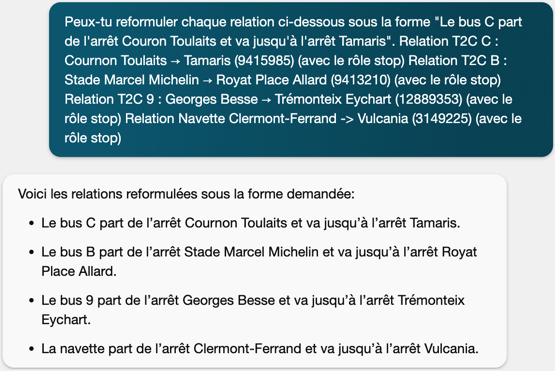
\includegraphics[width=0.6\textwidth]{images/conclusion/test_gpt.png}
    \caption[Mise en forme textuelle avec GPT-4]{Exemple de mise en forme d'une donnée structurée en texte en utilisant GPT-4 (interface Bing Search en 2023).}
    \label{fig:conclusion_testgpt}
\end{figure}